\documentclass{article}
\usepackage{mathtools}
\usepackage{graphicx}
\usepackage{hyperref}
\usepackage{subcaption}
\usepackage[slovak]{babel}

\hypersetup{
    colorlinks=true,
    linkcolor=blue,
}

\graphicspath{ {./img/} }

\title{PB170 -- ALU}
\author{Ondrej Klinovský, Jakub Maloštík}

\begin{document}
    \maketitle

    \paragraph{}
    Cieľom tohto projektu bolo vytvoriť aritmeticko-logickú jednotku (ALU) so štyrmi operáciami. ALU pracuje so 4-bitovými číslami v doplnkovom kóde. Zvolili sme dve aritmetické operácie (sčítanie a odčítanie) a dve logické (logický súčin a súčet).
    \paragraph{}
    ALU sa ovláda pomocou dvoch tlačítiek a ôsmych prepínačov. Prepínače predstavujú vstup pre dve 4-bitové čísla. Operáciu nad tymíto číslami je možné zvoliť s dvomi tlačítkami následovne:
    \begin{center}
    \begin{tabular}{| c | c | c |}
        \hline
        X & Y & operácia \\
        \hline
        0 & 0 & sčítanie \\
        0 & 1 & odčítanie \\
        1 & 0 & logický súčin \\
        1 & 1 & logický súčet \\
        \hline
    \end{tabular}
    \end{center}
    Výstup ALU pozostáva zo štyroch LED-diód predstavujúcich výsledok zvolenej operácie a troch LED-diód predstavujúcich príznaky operácie: nulový výsledok, záporný výsledok a pretečenie aritmetickej operácie.

    \begin{figure}[h!]
        \centering
        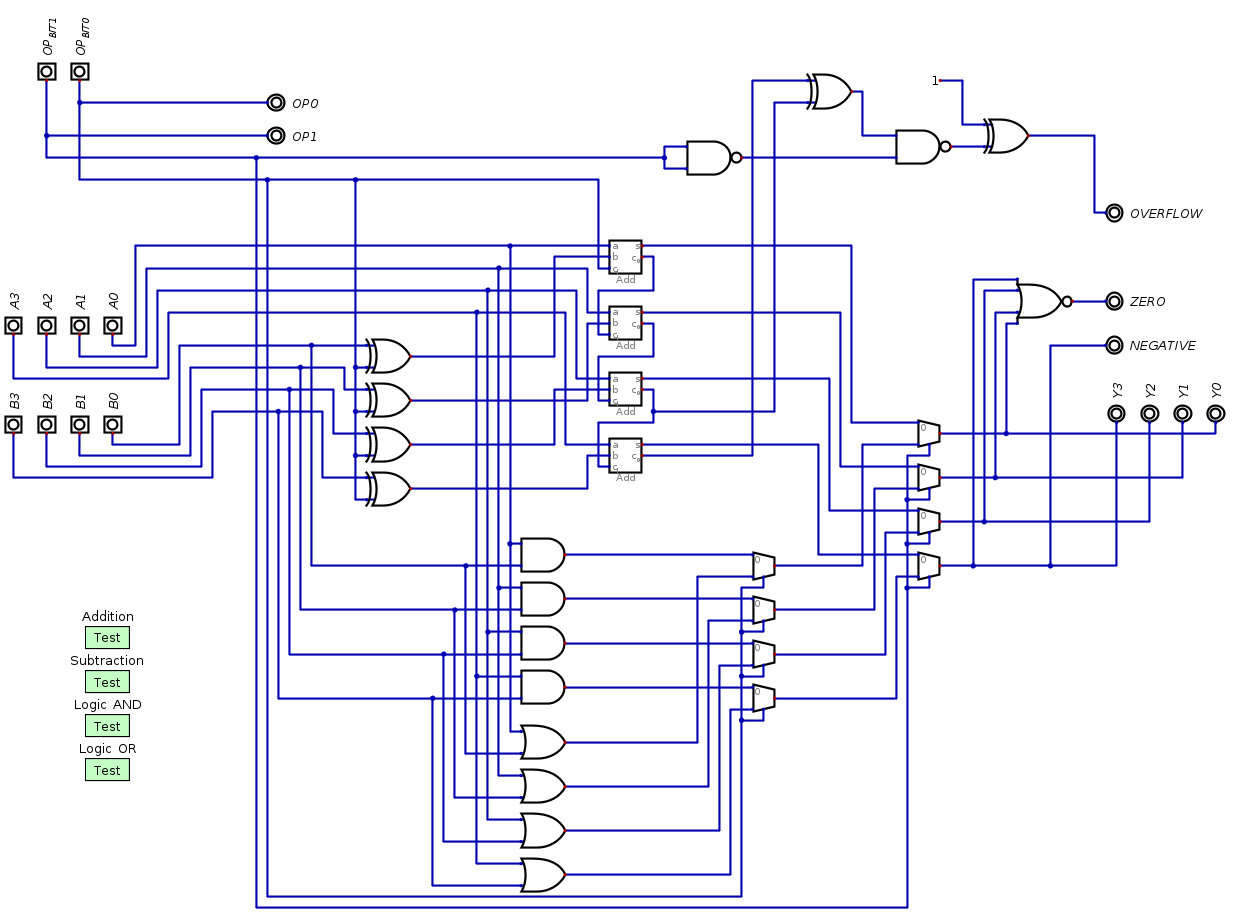
\includegraphics[width=.9\linewidth]{sim.png}
        \caption{Prvotný návrh sme spravili v simulátore digitalnych obvodov Digital. Na obázku je vidieť celá shéma obvodu ALU. Pre zjednodušenie návrhu sme použili vstavané komponenty ako sčítačky alebo multiplexer. Vstupy su riešené jednoduchými prepínačmi.}
    \end{figure}

    \paragraph{}
    Celý obvod sme si rozdelili na tri časti: vstup, výstup a samotná ALU. Výstup je najjednoduchšia časť, tvorí ho sedem LED-diód reprezentujúcich 4-bitový výsledok a tri príznaky. Výstup je o niečo zložitejší. Nachádzajú sa tu dve tlačítka napojené na D klopné obvody, vďaka ktorým sme schopní meniť operáciu ALU. Osem prepínačov slúži pre zadávanie dvoch 4-bitových čísel pre ALU. Na každý vstup je napojená jedna LED-dióda pre zobrazenie dát, s ktorými ALU pracuje.

    \begin{figure}[h!]
        \centering
        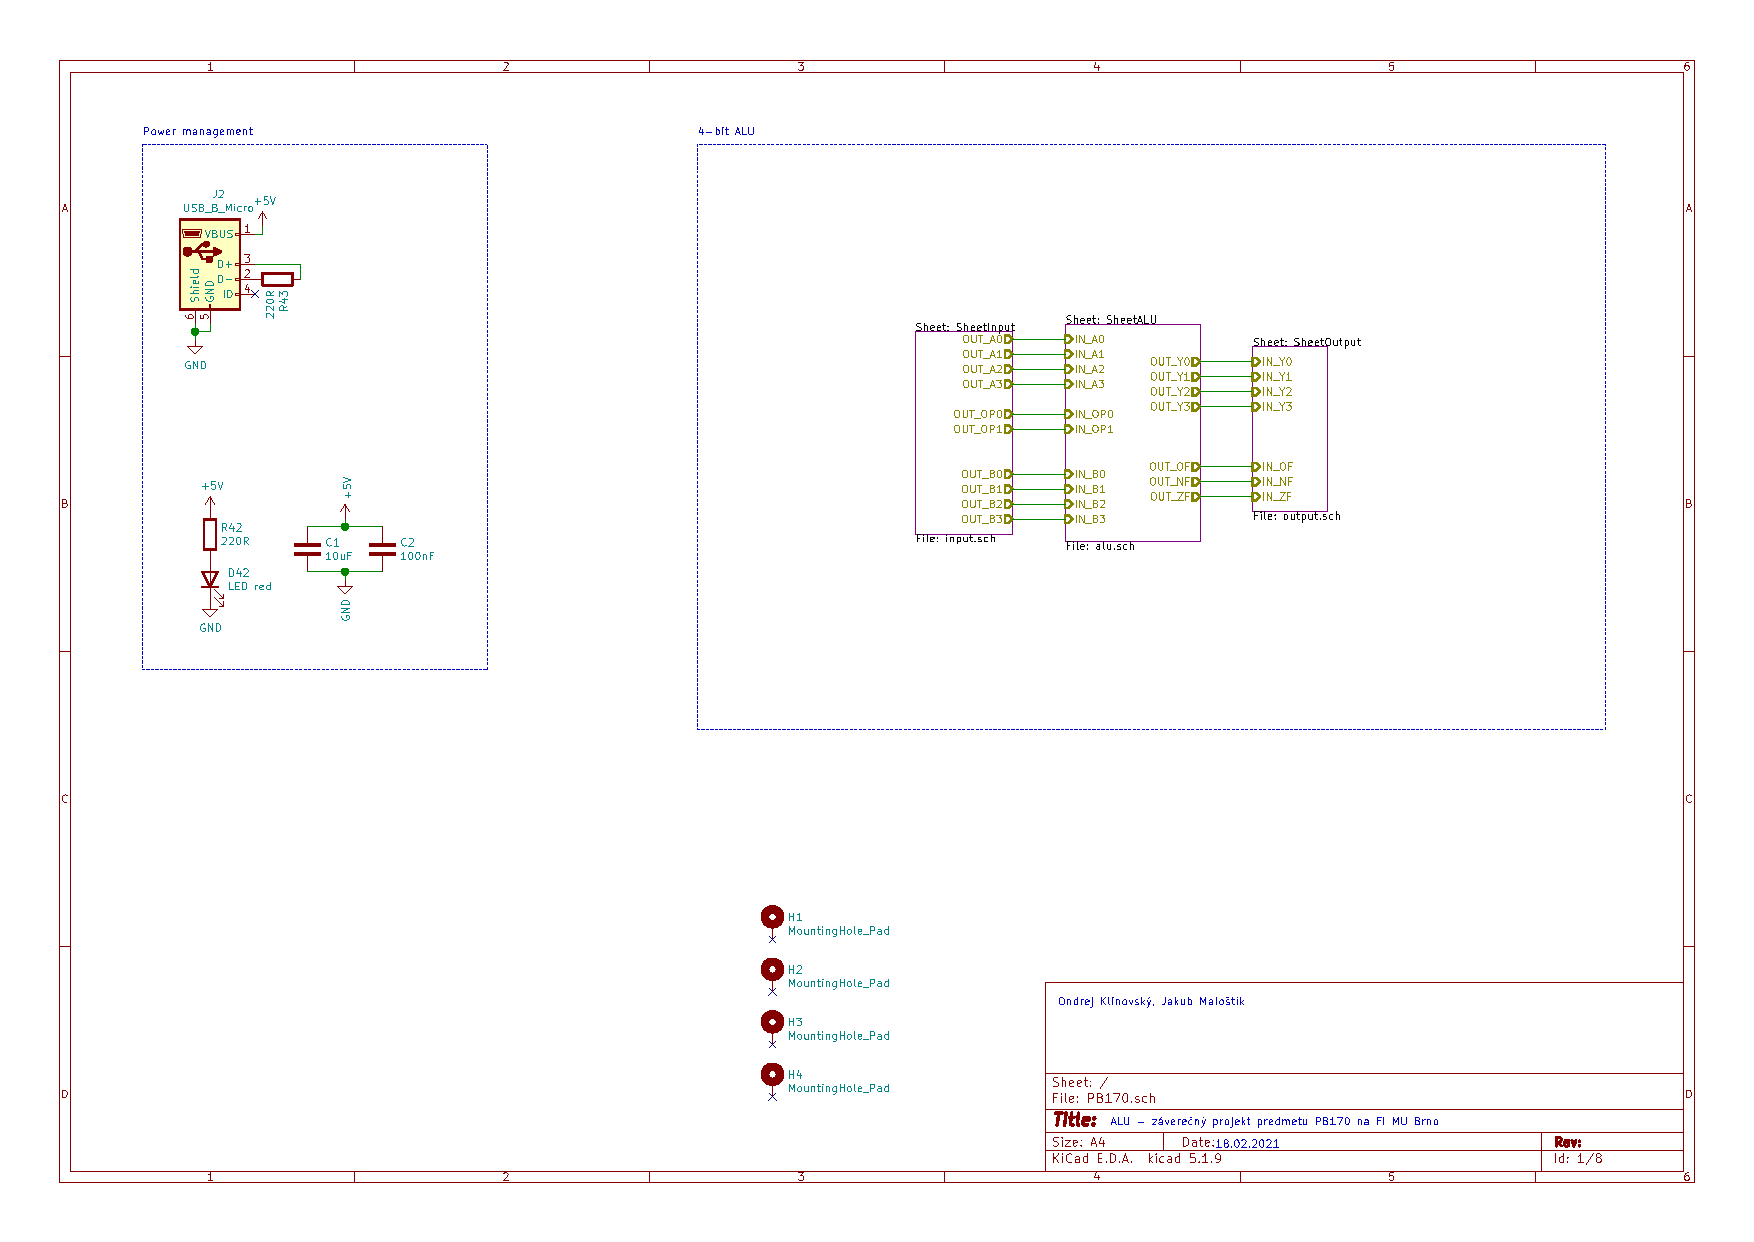
\includegraphics[width=.9\linewidth]{top_sheet.pdf}
        \caption{Na tejto schéme môžme vidieť vľavo napájanie obvodu (prevziate z poskytnutej šablóny) a vpravo samotný obvod rozdelený na tri podschémy, zľava: vstup, ALU a výstup.}
    \end{figure}

    \begin{figure}[h!]
        \centering
        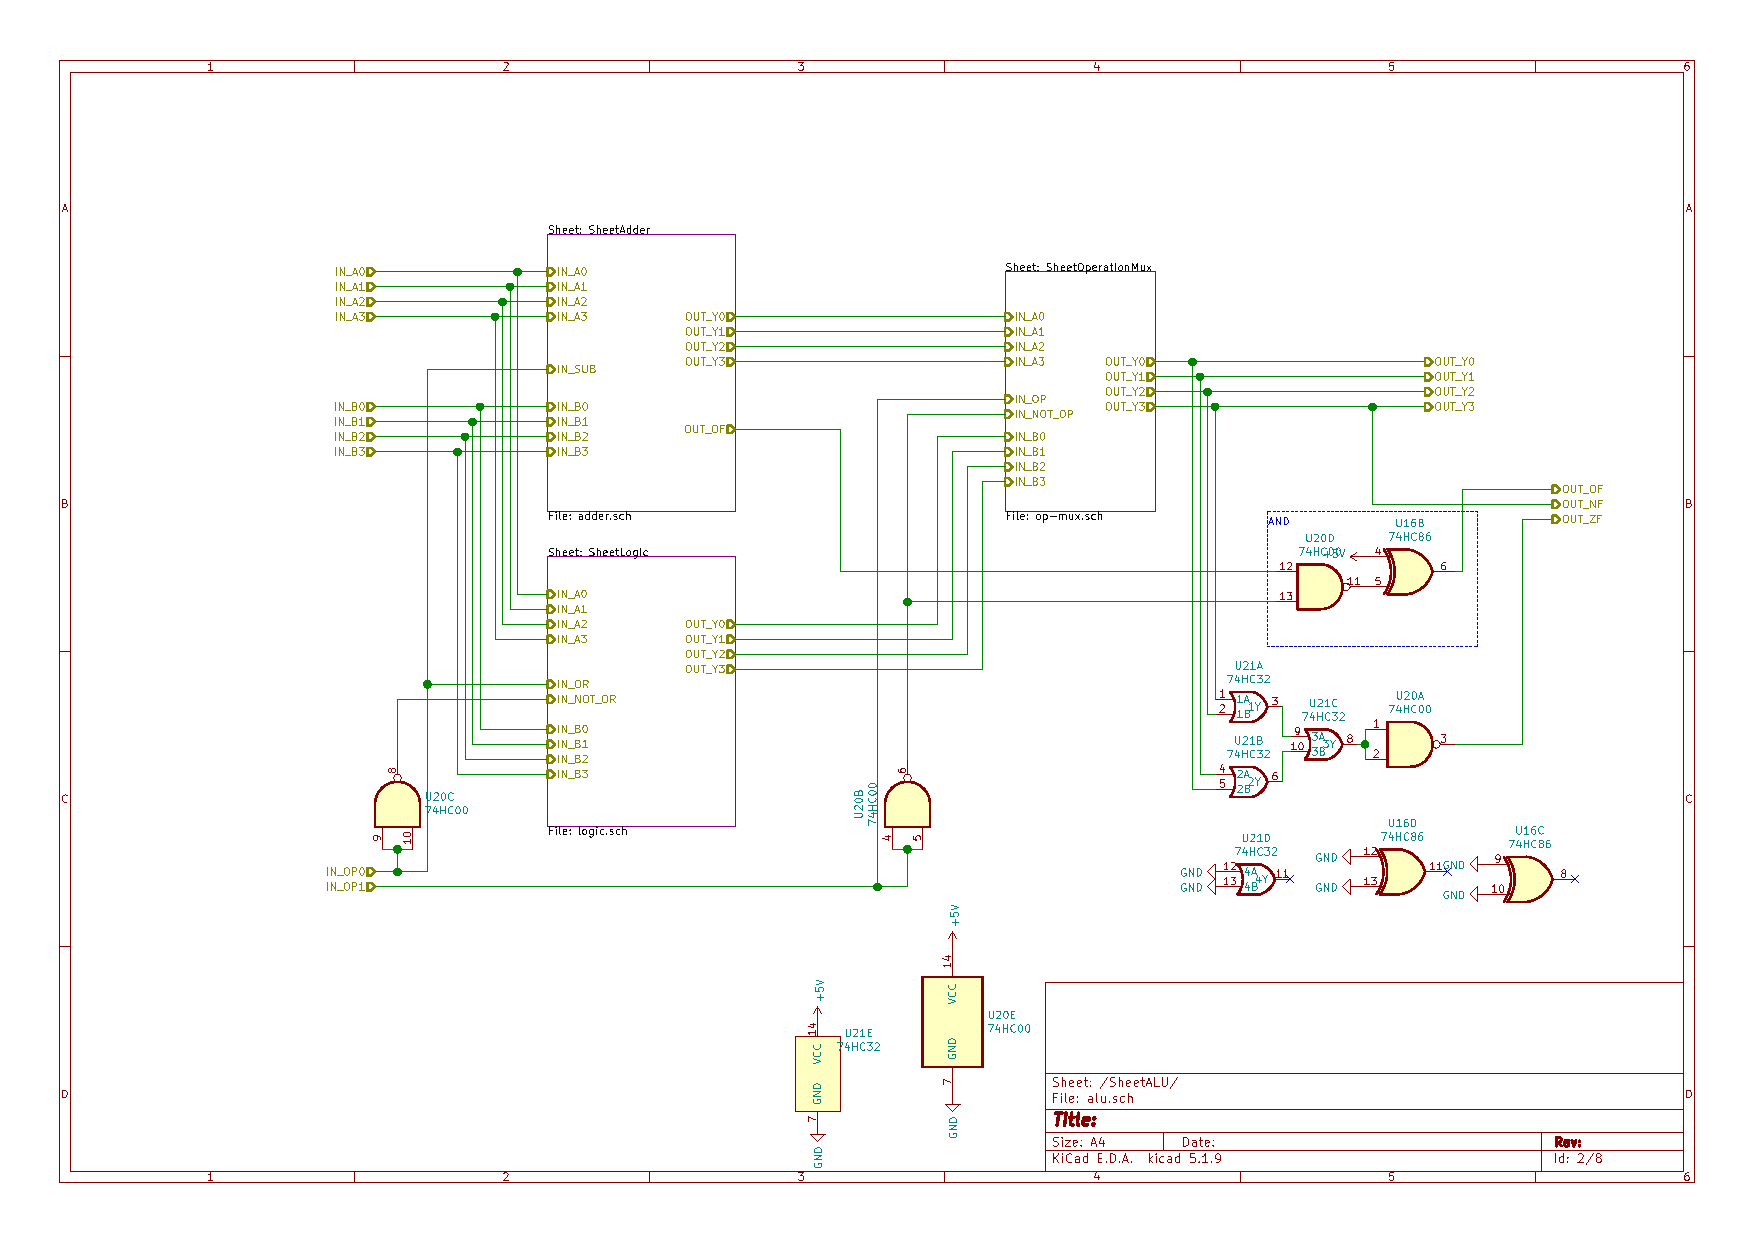
\includegraphics[width=.9\linewidth]{alu_sheet.pdf}
        \caption{}
    \end{figure}

    \begin{figure}[h!]
        \centering
        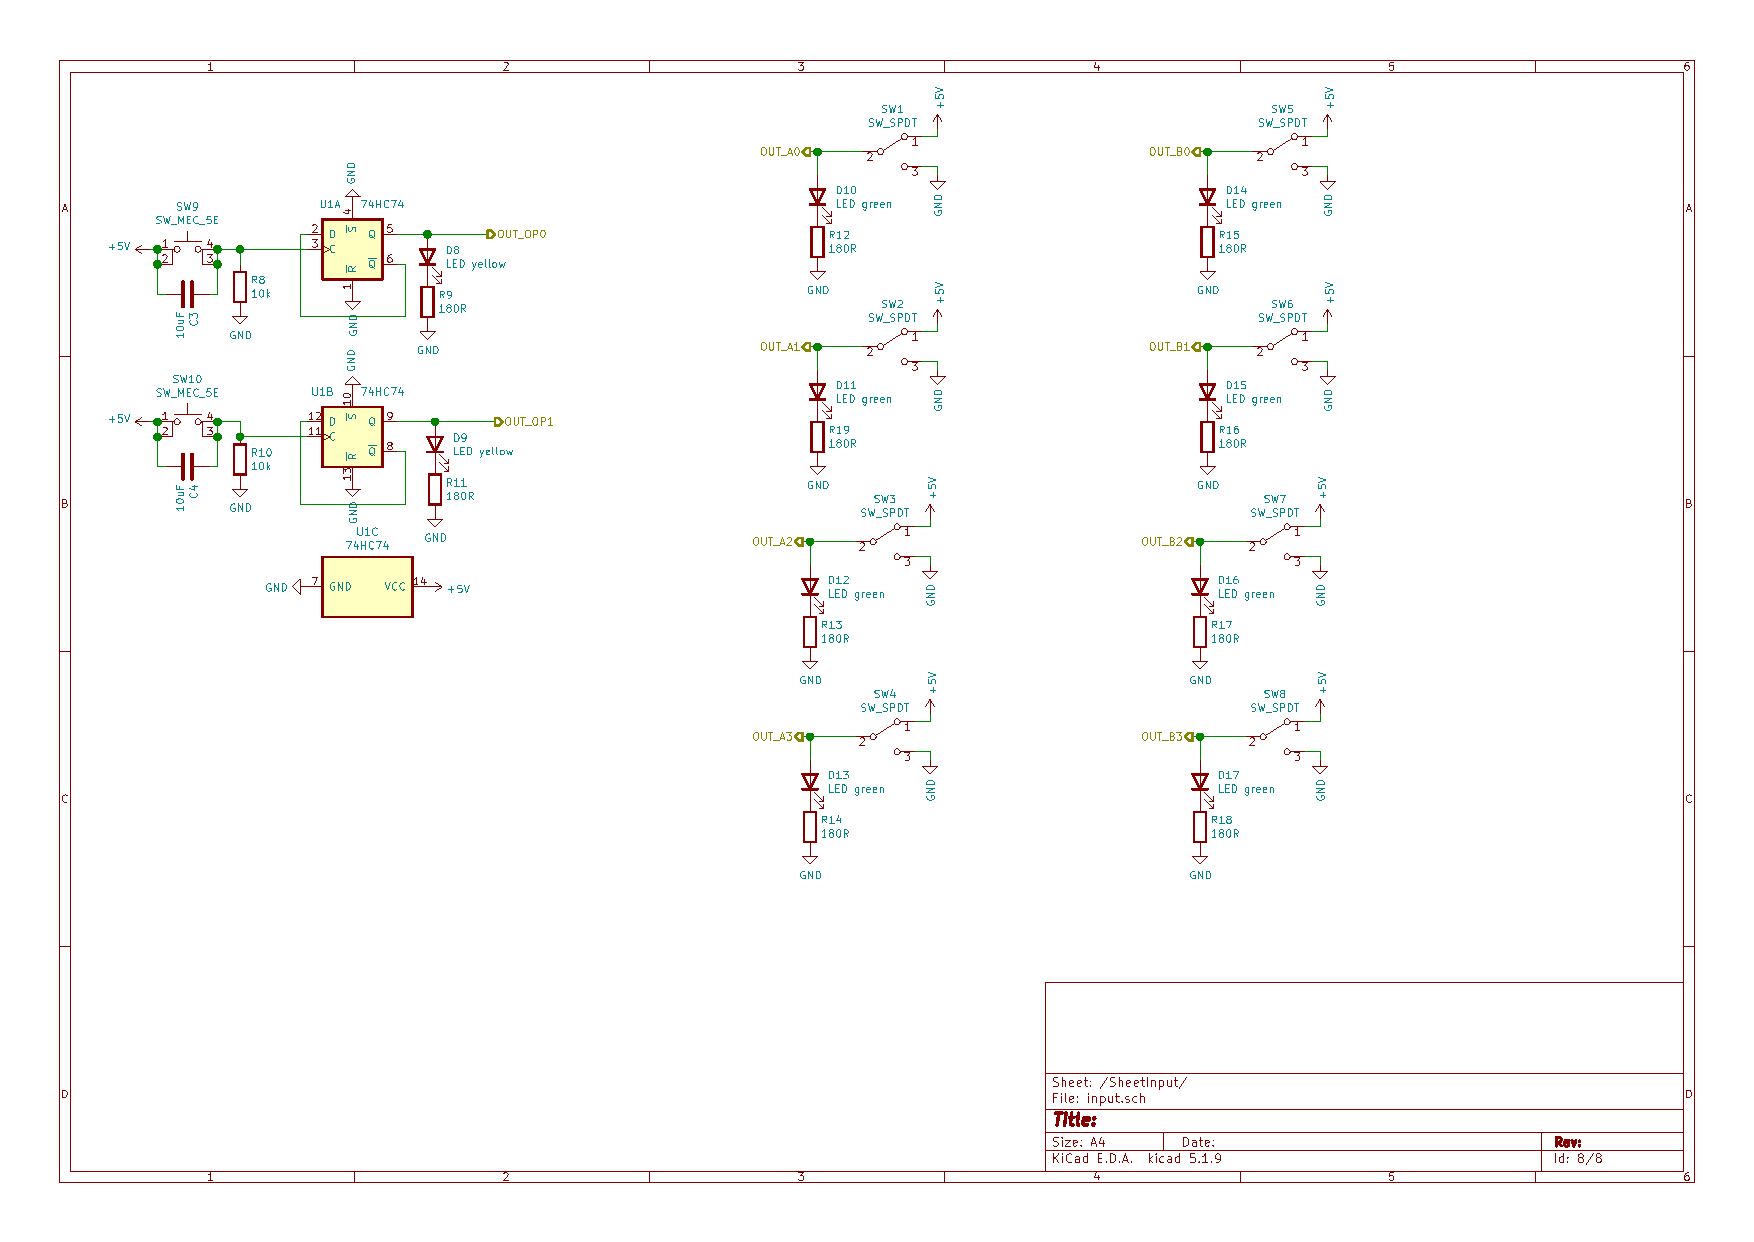
\includegraphics[width=.9\linewidth]{input_sheet.pdf}
        \caption{Vľavo sa nachádzajú dve tlačítka s klopnými obvodmi D pre zadavanie operácie a napravo od nich osem prepínačov pre čísla A a B.}
    \end{figure}

    \begin{figure}[h!]
        \centering
        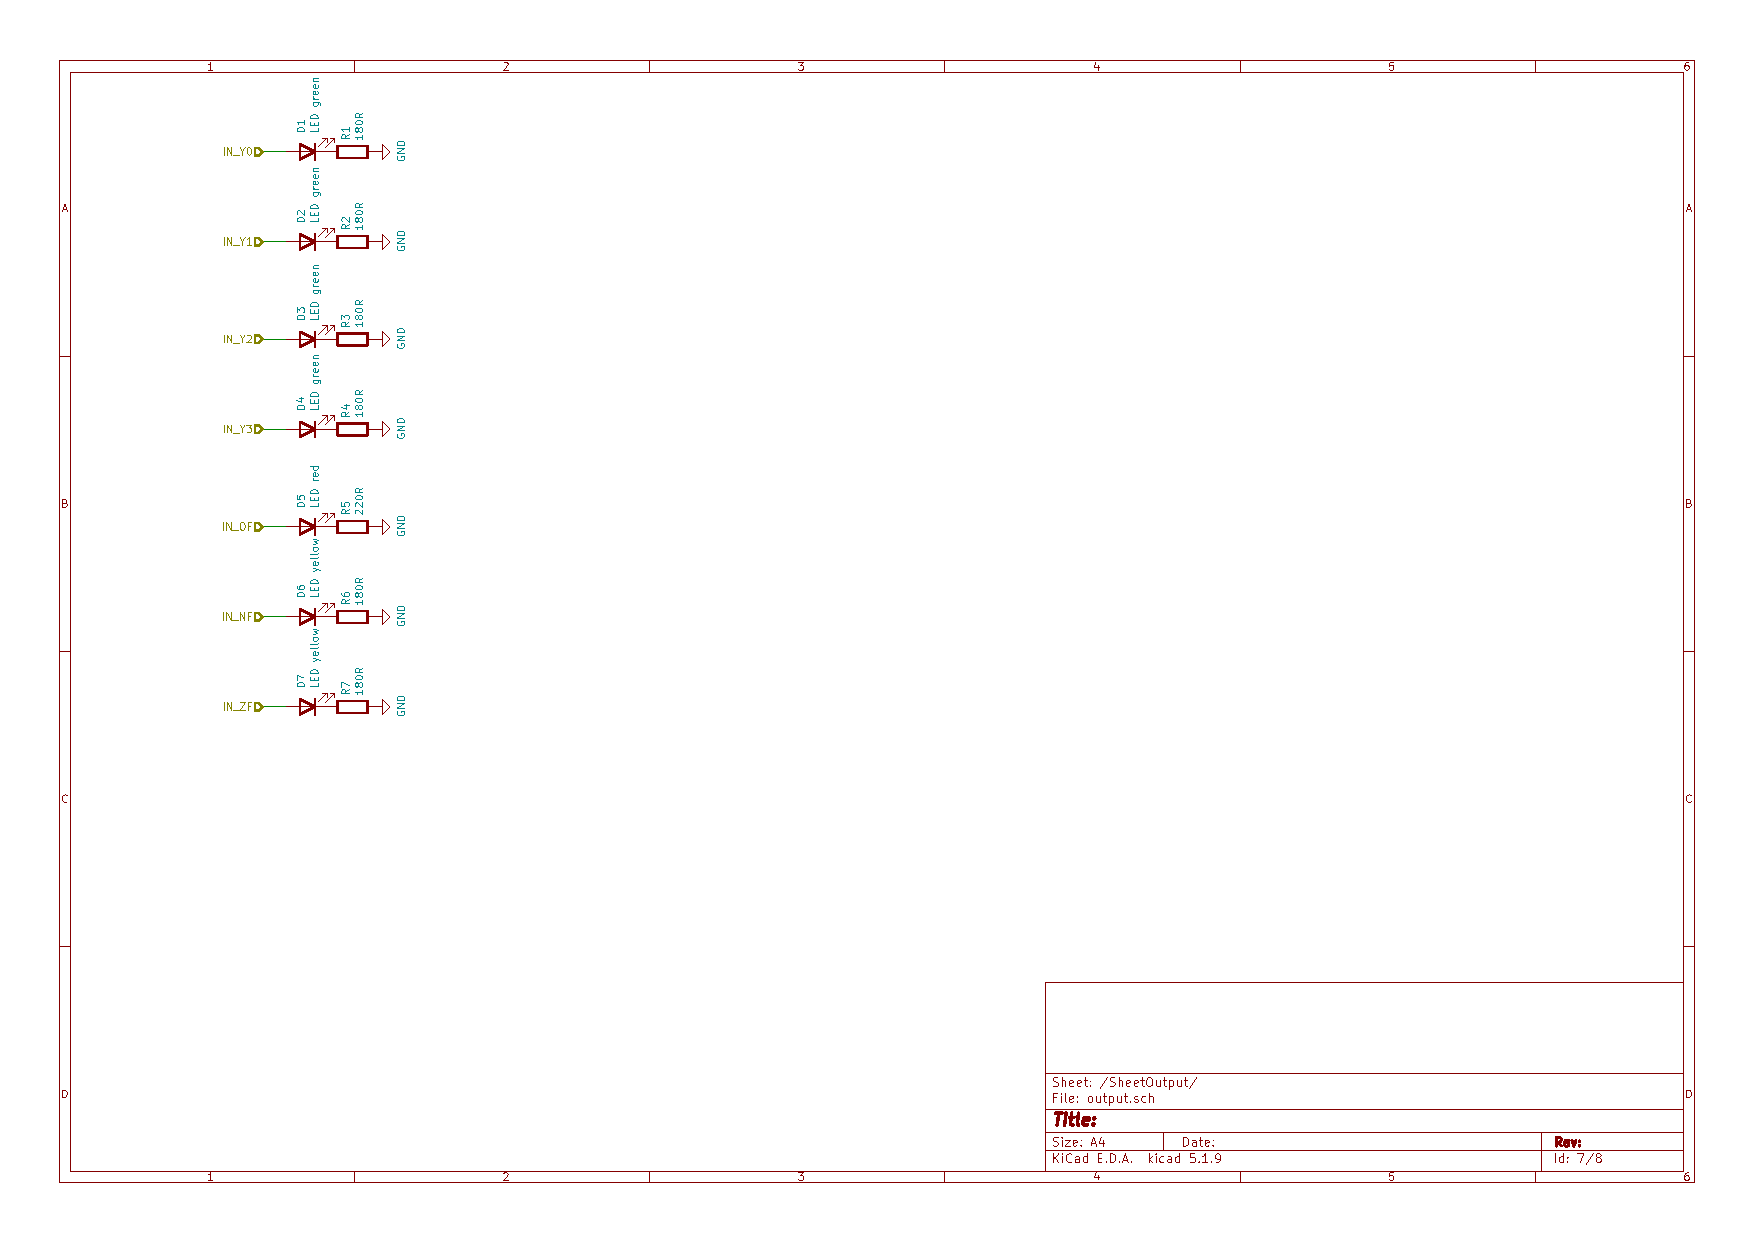
\includegraphics[width=.9\linewidth]{output_sheet.pdf}
        \caption{Štyri horné LED predstavujú výsledok operácie a tri LED pod nimi predstavú príznaky pretečenia, negatívneho výsledku a nulového výsledku.}
    \end{figure}

    \paragraph{}
    Treťou, najkomplikovanejšou časťou je ALU, ktorá sa pozostáva z aritmetickej (sčítačky) a logickej časti, multiplexeru a logiky pre zobrazenie príznakov. Mutliplexer na základe významnejšieho bitu operácie rozhoduje, či na vstup pošle výsledok aritmetickej alebo logickej časti. Obe majú na vstupe dve 4-bitové čísla a operačný bit (menej významný bit operácie) a na výstupe 4-bitový výsledok. V logickej časti sa nachádzajú štyri AND brány a štyri OR brány smerujúce do multiplexeru, ktorý na základe operačného bitu rozhodne, ktorý výsledok pošle na výstup. V aritmetickej časti nie je multiplexer potrebný. Odčítanie je možné previesť inverziou bitov čísla B a pripočítanie jednotky k výsledku. Inverzia bitov je implementovaná pomocou XOR brány. Zatiaľ čo číslo A na napojené priamo na sčítačku, číslo B prechádza cez XOR brány, kde tvorí vstup spolu s operačným bitom. Ak je operačný bit 0 (sčítanie), číslo B prejde XORmi bez zmeny. V prípade odčítania (operačný bit má hodnotu 1) XOR invertuje všetky bity čísla B. Pripočítanie jednotky je docielené tým, že operačný bit je napojený na carry-in vstup sčítačky. V prípade sčitovania bude mať carry-in hodnotu 0. Okrem 4-bitového čísla ma sčítačka na výstupe bit signalizujúci pretečenie, ktorý je výsledkom XOR operácie dvoch najvýznamnejších bitov výsledného čísla.

    \begin{figure}[h!]
        \centering
        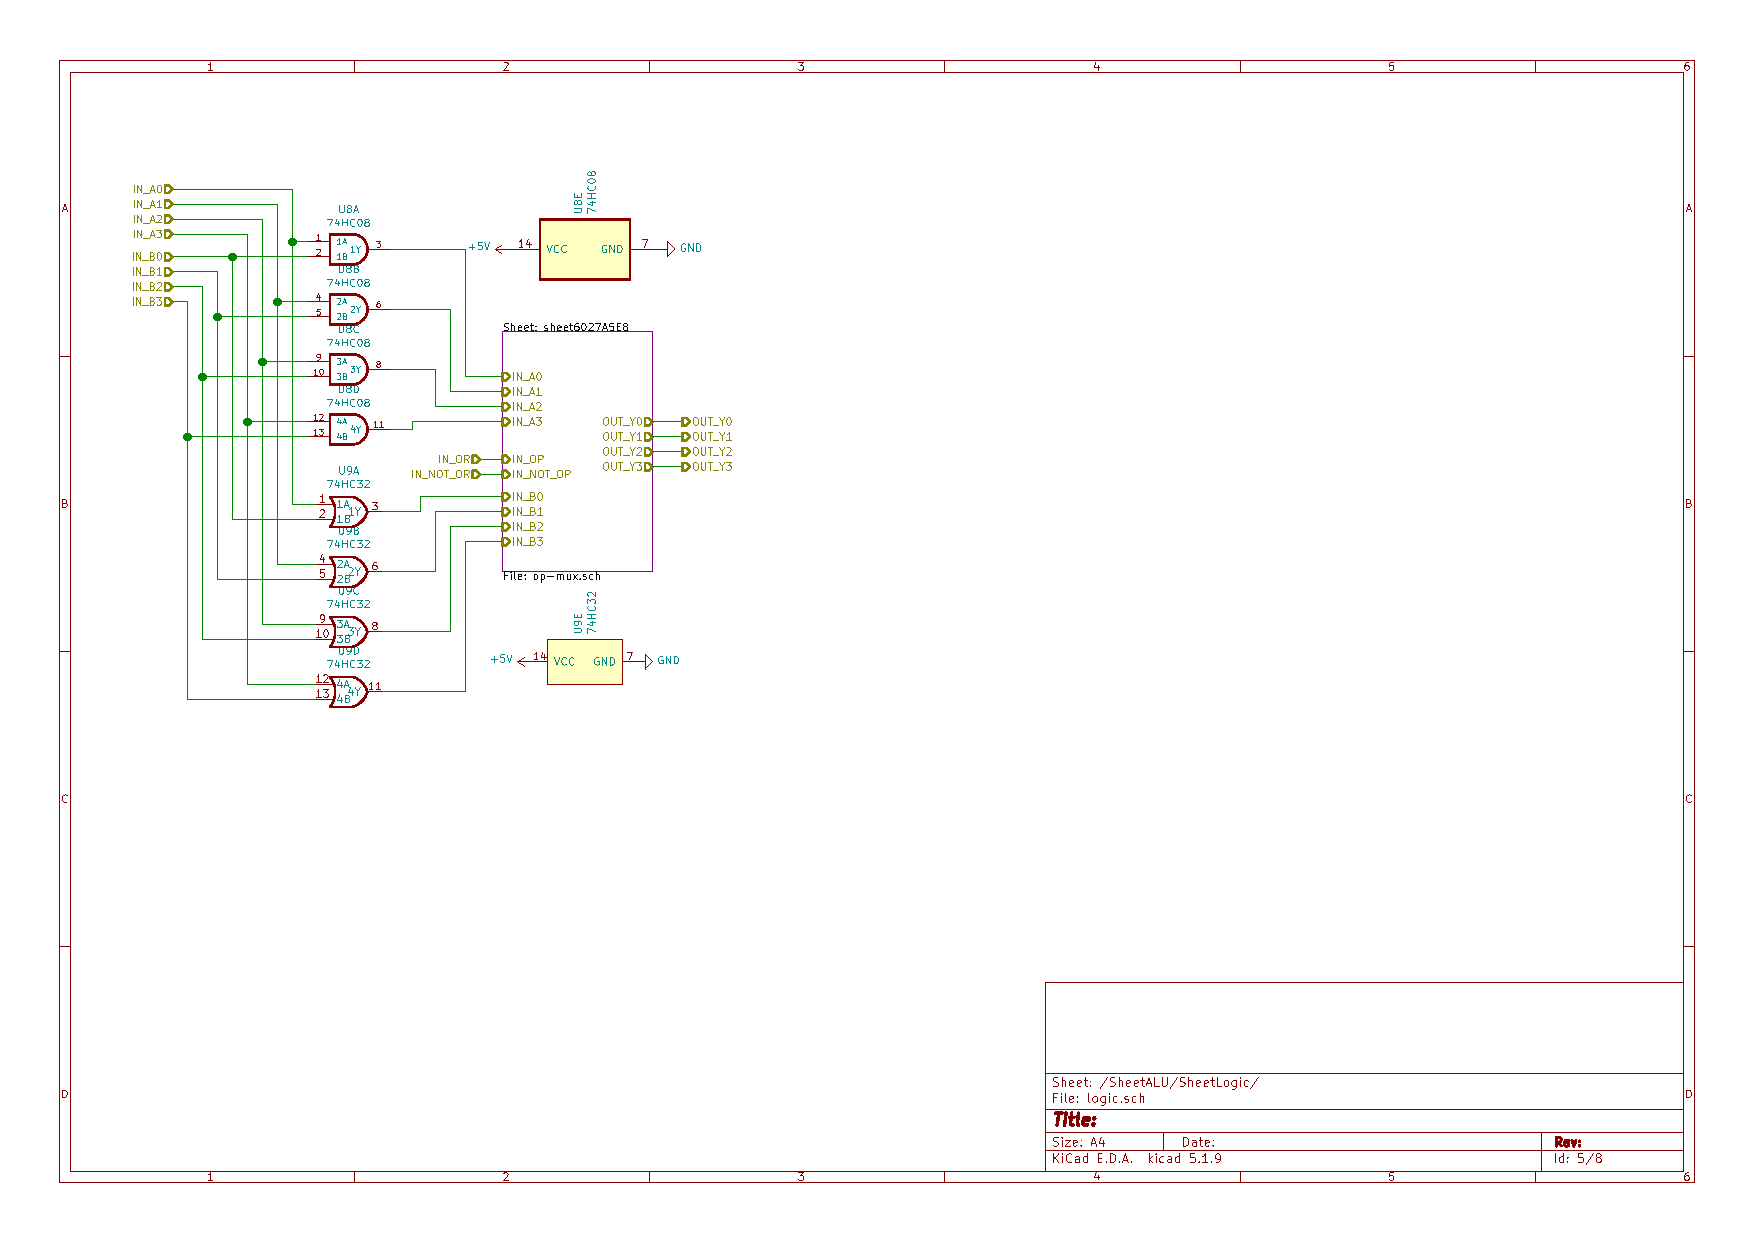
\includegraphics[width=.9\linewidth]{logic_sheet.pdf}
        \caption{todo}
    \end{figure}

    \begin{figure}[h!]
        \centering
        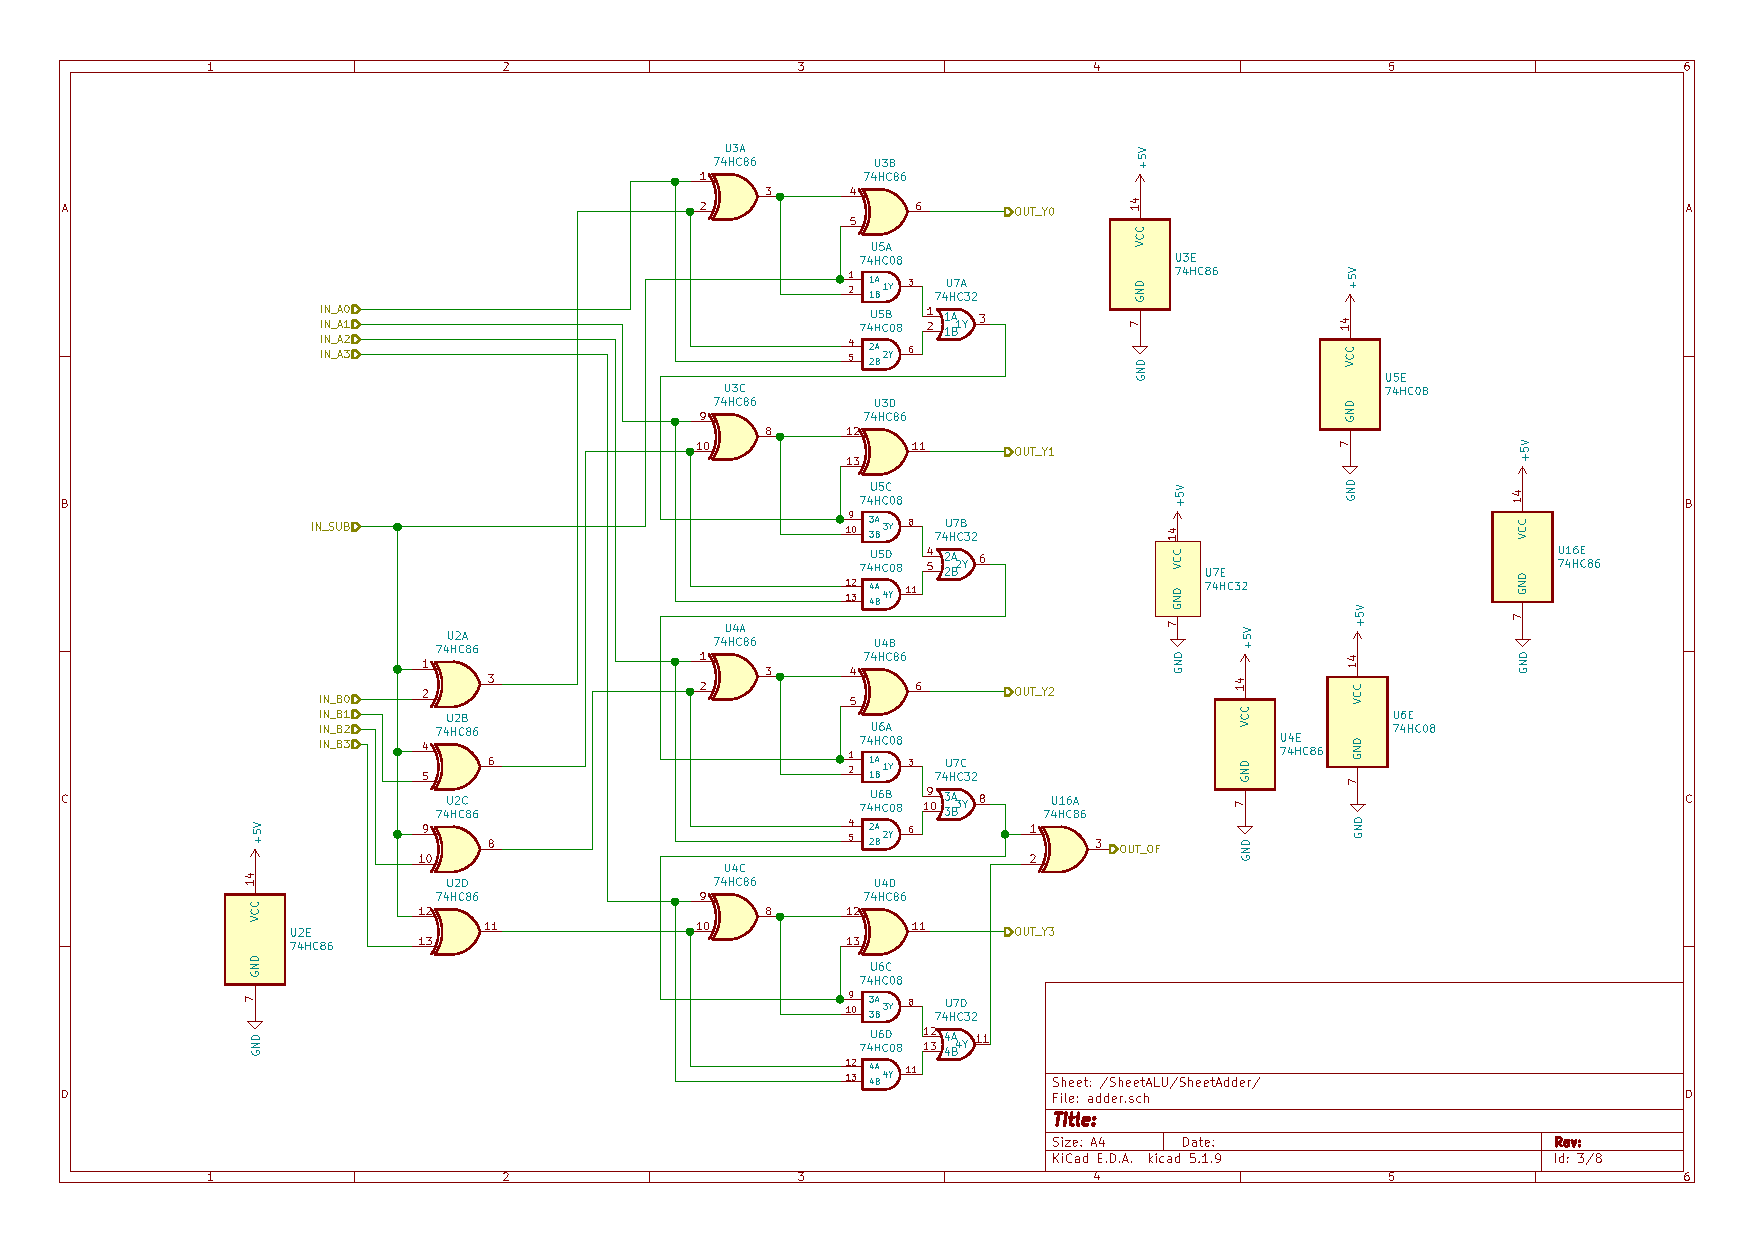
\includegraphics[width=.9\linewidth]{adder_sheet.pdf}
        \caption{Obvod pre sčítanie a odčítanie. Vľavo môžme vidieť štyri XOR brány pre prevracanie hodnôt čísla B, ktoré ďalej pokračujú do bitových sčítačiek. Výstupný signál OUT\_OF (príznak pretečenia) je výsledok operácie XOR, ktorej vstupom sú signály carry-out sčítačiek dvoch najvýznamnejších bitov.}
    \end{figure}

\end{document}

